\documentclass[
    % english, % Klasei padavus parametrą 'english', darbas bus anglų kalba.
    % signatureplaces % prideda parašų vietas tituliniame puslapyje
]{VUMIFPSbakalaurinis}
\usepackage{float}
\usepackage{wrapfig2}
\usepackage{hyperref}
\usepackage{algorithmicx}
\usepackage{algorithm}
\usepackage{algpseudocode}
\usepackage{amsfonts}
\usepackage{amsmath}
\usepackage{bm}
\usepackage{caption}
\usepackage{color}
\usepackage{graphicx}
\usepackage{listings}
\usepackage{subcaption}
\usepackage{biblatex}
\usepackage{framed,color,verbatim}
\usepackage{dirtree}
\usepackage[table]{xcolor}% http://ctan.org/pkg/xcolor
\definecolor{shadecolor}{rgb}{.9, .9, .9}
\usepackage{tabularx}
\newcolumntype{L}{>{\raggedright\arraybackslash}X}


% Titulinio aprašas
\university{Vilniaus universitetas}
\faculty{Matematikos ir informatikos fakultetas}
\department{Programų sistemų bakalauro studijų programa}
\papertype{Bakalauro baigiamasis darbas}
\title{Kodo skirstymo į paketus šablonų tyrimas}
\titleineng{Analysis of code packaging patterns}
\author{Martyna Ubartaitė}
% \secondauthor{Vardonis Pavardonis}   % Pridėti antrą autorių
\supervisor{Gediminas Rimša}
\reviewer{doc. dr. Audronė Lupeikienė}
\date{Vilnius – \the\year}

\bibliography{bibliografija}

\begin{document}
\maketitle

%% Padėkų skyrius
% \sectionnonumnocontent{}
% \vspace{7cm}
% \begin{center}
%     Padėkos asmenims ir/ar organizacijoms
% \end{center}

\begin{lithuanian}
\sectionnonumnocontent{Santrauka}
Glaustai aprašomas darbo turinys: pristatoma nagrinėta problema ir padarytos
išvados. Santraukos apimtis ne didesnė nei 0,5 puslapio. Santraukų gale
nurodomi darbo raktiniai žodžiai. Automatiškai naudojamos lietuviškos kabutės: \enquote{tekstas}.

% Nurodomi iki 5 svarbiausių temos raktinių žodžių (terminų).
% Vienas terminas gali susidėti iš kelių žodžių.
\raktiniaizodziai{raktinis žodis 1, raktinis žodis 2, raktinis žodis 3, raktinis žodis 4, raktinis žodis 5}
\end{lithuanian}

\begin{english}
\sectionnonumnocontent{Summary}
Santrauka anglų kalba. Santraukos apimtis ne didesnė nei 0,5 puslapio. Automatiškai naudojamos angliškos kabutės: \enquote{tekstas}.

\keywords{keyword 1, keyword 2, keyword 3, keyword 4, keyword 5}
\end{english}

\tableofcontents

\sectionnonum{Įvadas}
\subsection{Problema ir jos aktualumas}
Teisingai įgyvendintas kompiuterinės sistemos dizainas yra vienas iš kritinių sėkmingo verslo
elementų.
Tam, jog verslas išlaikytų stabilų augimą yra būtina sukurti sistemą, kuri sumažintų
atotrūkį tarp organizacijos tikslų ir jų įgyvendinimo galimybių.
Mąstant apie programinio kodo
dizainą, kodo paketų kūrimas, klasių priskyrimas jiems ir paketų hierarchijos sudarymas paprastai
nėra pagrindinis prioritetas, tačiau tai parodo praleistą galimybę padaryti sistemos dizainą labiau
patikimu[Sho19], suprantamu [Eli10] ir lengviau palaikomu.
Modernios sistemos yra didžiulės, programinis kodas yra padalintas į daugybę failų,
kurie išskaidyti per skirtingo gylio direktorijas, todėl apgalvotai išskirstytas programinis
kodas daro daug didesnę įtaką kodo kokybei, nei gali atrodyti iš pirmo žvilgsnio.
Sistemos paketų studijavimas ir analizė norint įvertinti programinės įrangos kokybę
tampa vis svarbesne tema, dėl pastoviai augančio failų ir paketų skaičiaus\cite{DesignMetrics}.


Norint išsiaiškinti, kaip efektyviausiai gali būti skaidomas programinis
kodas, tam jog jo struktūra darytų teigiama įtaką sistemos kokybei, reikalinga atlikti skirstymo į paketus šablonų analizę -
išsiaiškinti galimus šablonus ir būdus, kaip skirstyti programinį kodą į paketus, turėti aiškius šablonų apibrėžimus su jų
privalumai bei trūkumais.

\subsection{Darbo tikslas}
Šio darbo tikslas - identifikuoti šablonus kodo skirstymui į paketus.
Remiantis moksliniais straipsniais apie sistemos kokybę bei palaikomumą aprašyti kriterijus,
kurie būtų naudojami šablonus įvertinti, nustatant jų įtaką sistemos palaikomumui.

\subsection{Keliami uždaviniai}
\begin{itemize}
    \item Išskirti gerai įgyvendinto kodo požymius
    \item  Aprašyti skirstymo į paketus šablonus, remiantis pavyzdžiais teorinėje medžiagoje bei
egzistuojančiose atviro kodo sistemose
    \item  Įvertinti kiek realių sistemų struktūra nutolusi nuo teorinių šablonų apibrėžimų
    \item  Pasiūlyti kriterijus, įvertinančius kodo suskirstymo šablono įtaką sistemos kokybei, remiantis
rastai gerai įgyvenditos sistemos požymiais
    \item  Pasirinkti kelias sistemas ir pertvarkyti jų failų struktūrą pagal aprašytus šablonus, įvertinant
kiek sudėtinga pasiekti kiekvieno šablono strukūrą
    \item  Naudojant pertvarkytas sistemas, įvertinti kiekvieną kodo skirstymo šabloną pagal pasiūlytus kriterijus
    \item  Pateikti rekomendacijas, kokius šablonus kodo skirstymui tinkamiausia naudoti
\end{itemize}
todo: apubidinti šaltinius
todo: aprašyti kas yra šablonai
todo: pamineti praktine dalį

\subsection{Numatomas darbo atlikimo procesas}
\begin{itemize}
    \item Remiantis teorine medžiaga aprašomi gerai įgyvendinto kodo požymiai, užtikrinantys
sistemos stabilumą ir palaikomumą.
    \item Aprašomi kriterijai, kuriuos naudojant galima įvertinti kodo suskirstymo įtaką sistemos
kodo kokybei, pavyzdžiui:
    \begin{itemize}
        \item Komponentų skaičius, priklausomas nuo pasirinkto komponento[Mah03]
        \item Tiesioginės ir netiesioginės priklausomybės (matomumas)[Ala07]
    \end{itemize}
    \item Galimų kodo skirstymo šablonų išskyrimas pasitelkiant teorinę informaciją [Sho11] ir
egzistuojančių sistemų architektūrą.
    \item Atviro kodo projektų pasirinkimas. Pasirenkami skirtingo tipo projektai, užtikrinant
objektyvesnę šablonų analizę skirtingose srityse. Galimi tipai:
    \begin{itemize}
        \item Taikomoji programinė įranga, teikianti paslaugas įrangos naudotojams. Pavyzdžiui,
internetinė programėlė priminimams ir darbams užsirašyti
        \item Techninė programinė įranga, naudojama taikomosios programinės įrangos duomenų
saugojimui, siuntimui, paieškai. Pavyzdžiui, duomenų bazės, pranešimų eilės, talpyklos
(angl. cache)
        \item Programinės įrangos įrankiai, skirti naudoti kitose sistemose supaprastinant programinį
kodą, naudojant jau įgyvendintas funkcijas. Pavyzdžiui, Java programavimo kalbos
Spring karkasas internetinių programėlių kūrimui
    \end{itemize}
    \item Pasirinktų projektų paketų sturktūros pertvarkymas pagal pasirinktus skirstymo šablonus
    \item Pertvarkytų projektų įvertinimas, naudojant išskirtus kriterijus, nustatant, kokią įtaką
skirtingi skirstymo šablonai turi sistemos kokybei
\end{itemize}


\subsection{Laukiami rezultatai}
\begin{itemize}
    \item Įdentifikuoti kodo skirstymo šablonai, remiantis teorine informacija ir praktikoje sutinkamais pavyzdžiais
    \item Sukurti kriterijai, įvertinantys sistemos paketų struktūros indėlį sistemos kokybei
    \item Pasirinkti projektai pertvarkyti pagal kodo skirstymo šablonus
    \item Įvertinus šablonus sukurtais kriterijais, pateiktos rekomendacijos kodo skirstymo šablonų naudojimui
\end{itemize}


\subsection{todo:}
aprašyti sekančius chapterius.
\section{Galimi kodo skirstymo į paketus šablonai}
Diskusijose, kaip reikėtų skirstyti programini kodą, paprastai akcentuojami du šablonai - pagal \textit{techninį sluoksnį}, todo: šaltiniai, nurodantys skirstymo būdus
kur kiekvienam funkcionalumui arba kompiuterinės sistemos sluoksniui yra sukuriamas paketas,
grupuojant skirtingų dalykinių sričių esybes, arba pagal \textit{dalykinės srities esybes}, kur vienos esybės kodas, dalykinės srities
esybės funkcionalumas skirtingose programiniuose sluoksniuose yra patalpintas viename pakete.
Tačiau šie du šablonai yra gan platūs ir galėtų būti išskaidyti į daugiau smulkesnių ir tiksliau aprašytų šablonų.
Taip pat, minėtuose šablonuose, būdai kaip ir kodėl skaidyti programinį kodą parinkti akecentuojant tai, kaip programinį
kodą supranta žmonės, dirbantys prie to kodo.
Nuspresti, kaip žmones supranta programinį kodą yra gan sudėtingas ir subjektyvus procesas, todėl aprašant šablonus, kodo skirstymui
geriau akcentuoti, kaip sugrupuoti paketai bendrauja tarpusavyje ir skirstyti juos pagal klasių naudojimo atvejus ir priklausomybes.
Taip kodo grupavimo metodai yra labiau artimi Martino aprašytiems principams.


Šablonus kaip grupuoti kodą, akcentuojant klasių naudojimo atvejus ir priklausomybes nagrinėja Martin Sandin savo
straipsnyje \textit{Four Strategies for Organizing Code}.
Šis straipsnis idomus tuo, kad autorius nesiplečia į du dažniausiai sutiknamus šablonus - grupuoti pagal techninį sluoksni arba dalykinės srities esybes,
o aprašo keturis grupavimo būdus arba šablonus, kurie, nors ir įkvėpti minėtų dviejų budų, yra gan unikalūs ir labiau techniškai apibrėžti.
\subsection{Pagal komponentą}
Organizavimas pagal komponentus sumažina sistemos sudėtingumą, pabrėždamas išorinę ir vidinę kodo vienetų darną.
Išorinė darna reiškia, kad paketas turi minimalią sąsają \angl{interface}, kuri atskleidžia tik konceptus (metodus arba duomenų tipus),
kurie yra glaudžiai susijusios su komponento teikiama paslauga.
Vidinė darna reiškia, kad pakuotėje esantis kodas yra stipriai susijęs tarpusavyje ir susijęs su teikiama paslauga.

Kodas yra grupuojamas į mažus paketus, turinčius vieną, aiškiai apibrėžtą funkcionalumą ar tikslą, aprašant abstrakciją, kokie paketo elementai
yra pasiekiami iš išorės ir kaip jie naudojami.
Taip sukuriamas kodas, kuris yra lengviau suprantamas.
Tokį kodo grupavimo tcarką sunku palaikyti, tačiau jo rezultatas - kodas kuris yra lengviau suprantamas, lengviau pagerinamas, lengviau testuojamas
ir, dėl aiškiai aprašytų sąsajų, lengviau pernaudojamas.

\begin{figure}[H]
    \centering
    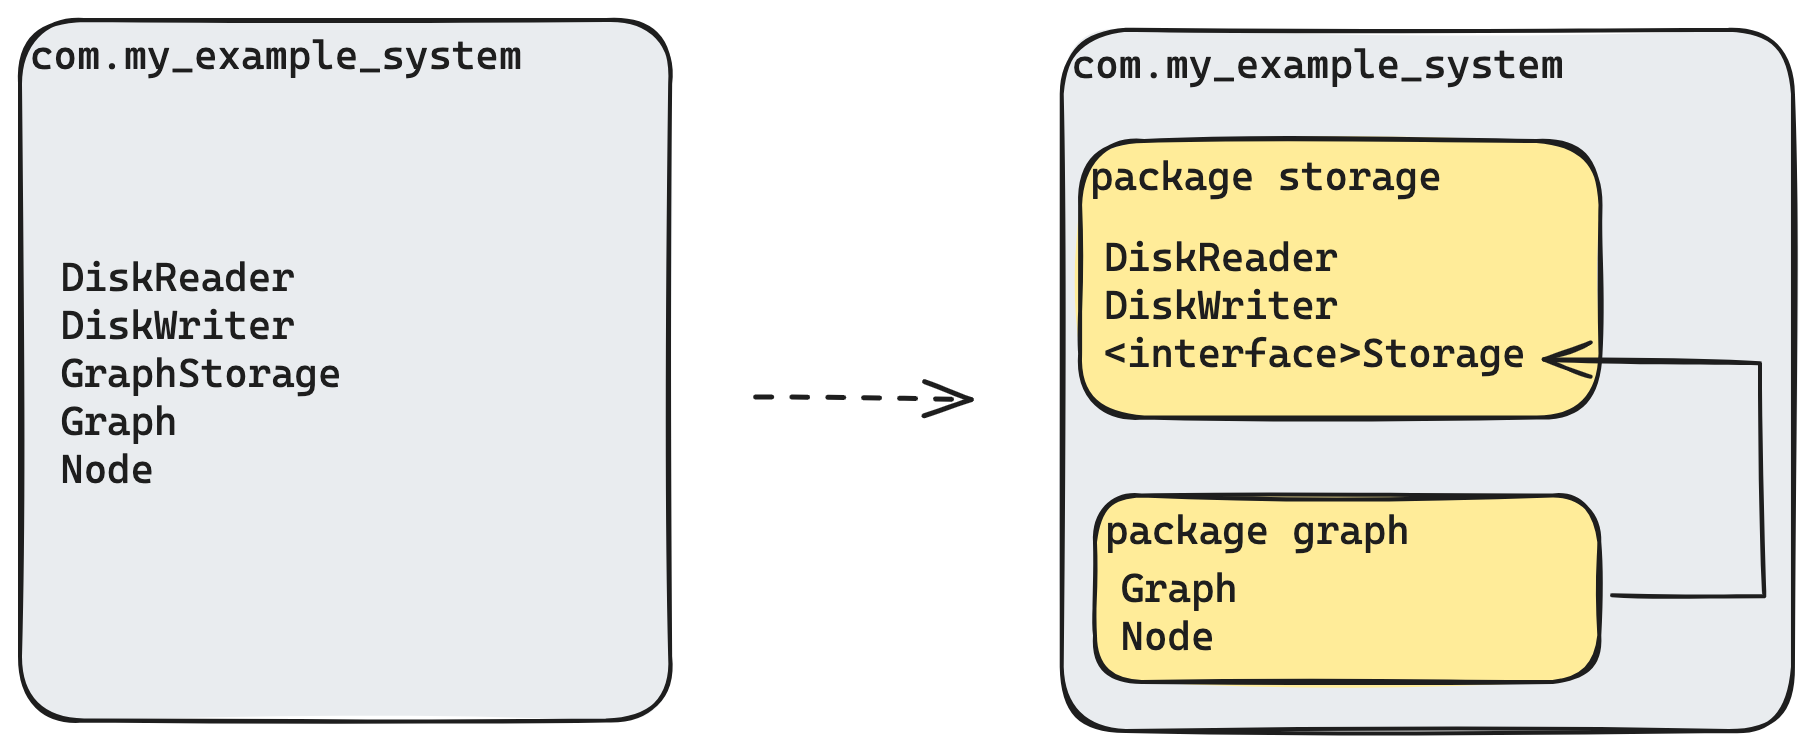
\includegraphics[scale=0.2]{img/component_packaging}
    \caption{Sistemos sugrupuotos pagal komponentą pavizdys}
    \label{img:component_packaging}
\end{figure}


\subsection{Pagal techninį sluoksnį}
\subsection{Pagal tipą}
\section{Kompiuterinės sistemos vertinimas}

\subsection{Teisingai įgyvendinta kompiuterinė sistema}
Norint išsiaiškinti, kokią įtaką sistemos kokybei daro skirtingos paketų skirstymo metodologijos ir kaip ojektyviai tą įtaką pamatuoti, pirmiausia
reikėtų apsibrėžti kokiais požymiais pasižymi teisingai įgyvendinta kompiuterinė sistema.
Martin Kleppmann savo knygoje \textit{Designing Data-Intensive Applications: The Big Ideas Behind Reliable, Scalable, and Maintainable Systems} išskyria šiuos pagrindinius kriterijus:
\begin{itemize}
    \item Patikimumas, reiškiantis, kad net ir klaidų (įrangos, programinių ar žmogiškųjų) atveju,
    sistema veikia stabiliai ir patikimai, paslepiant tam tikras klaidas nuo vartotojo\cite{DataIntensiveApplications}.
    \item Prižiūrimumas, reiškiantis jog skirtingų abstrakcijų pagalba sumažintas sistemos kompleksiškumas.
    Dėl to nesunku keisti esamą sistemos funkcionalumą bei pritaikyti naujiems verslo naudojimo atvejams.
    Tai supaprastina darbą inžinierių ir operacijų komandoms dirbančioms su šia sistema, taip pat leidžia prie sistemos prisidėti naujiems žmonėms, o ne
    tik jos ekspertams.
    Tai ypač aktualu atviro kodo sistemoms\cite{DataIntensiveApplications}.
    \item Plečiamumas, reiškiantis jog sistema turi strategijas, kaip išlaikyti gerą našumą užklausų
    srautui didėjant ir sistemai augant, tai atliekant su pagrįstais kompiuteriniais resursais ir
    priežiūros kaina\cite{DataIntensiveApplications}.
\end{itemize}
Yra daug skirtingų elementų, sudarančių sistemą, kuri tenkintų aukščiau paminėtus kriterijus,
pavyzdžiui, pasirinktos technologijos, aukšto lygio architektūra, dokumentacija, sistemos testavimo
procesai, jų kiekis ir pan.
Vienas iš svarbių elementų, prisidedančių prie gerai įgyvendintos sistemos dizaino yra programinio kodo dizainas, jo skaitomumas, patikimumas.
Konvencijos, kaip vadinti kodo paketus, kokias klasės jiems priskirti ir kokios paketų hierarchijos laikytis sudaro svarbią programinio kodo dizaino dalį,
Todėl programinės įrangos kurimo metu, laikas skirtas rasti sistemai tinkamą paketų skirstymo šabloną ir to šablono laikymasis atsiperka, padarant
programinį kodą geriau suprantamu, taip prisidėdant prie bendro sistemos dizaino patikimumo ir lengvesnio palaikomumo.

Straipsnyje \textit{Investigating The Effect of Software Packaging on Modular Structure Stability}, jo autoriai akcentuoja, kad
gerai įgyvendintos, objektiškai orientuotos sistemos turėtų vystytis be didelių pakeitimu jų architektūroje.
To siekiama todėl, nes architektūriniai pakeitimai paveikią didelę sistemos dalį ir todėl
jų įgyvendinimo ir priežiūros kaštai yra ženkliai didesni\cite{ModularStability}.
Paketų struktūra, kuri užtikrina atsieta (\angl{decoupled}) komunikavima tarp paketų, enkapsuliuoja paketų vidinius elementus, neleidžiant pakeitimais
išplisti už paketų ribų yra pagrindas tvirtai sistemos architektūrai, gebančiai efektyviai plėstis, ženkliai nesikeičiant ir sutaupant programos priežiūros kaštus.

\section{Įrankiai šablonų analizei ir įvertinimui}
Kompiuterinės sistemos, kurioms yra aktualu klasių ir paketų skirstymo metodai, paprastai yra labai didelės.
Pilnai perprasti tokias sistemas, nustatyti jų įgyvendinimo kokybę, naudojamus šablonus kodui skirstyti,
apskaičiuoti paketų kokybės matus yra sudėtingas procesas.
Daryti tai rankiniu būdu užtrunka daug laiko bei yra paliekama daug vietos potencialioms klaidoms,
todėl yra būtina šį procesą optimizuoti, skaitmenizuoti analizės procedūras pasitelkiant
 programinių įrankių pagalbą.

\subsection{Reikalavimai įrankiams}
Įrankių, leidžiančių paprasčiau atlikti sistemų analizę, atsakomybes galima suskirstyti į dvi grupes:
\begin{itemize}
    \item Bendrinė sistemos analizė - įrankis ar įrankiai padeda atlikti bendrinę sistemos analizę.
    Šios atsakomybių grupės įrankių išvestis nėra objektyvūs, tiksliai apibrėžtų formulių rezultatai, o papildoma, aiškiai
    pavaizduota meta informacija apie sistemą - paketų struktūrą, juose esančių klasių priklausomybes, dažnai pasikartojančius paketų bei klasių vardus.
    Ši papildoma informacija nėra aiškūs teiginiai, o tik pagalba analizę atliekančiams asmeniui, leidžianti priimti įžvalgas apie sistemą,
    kaip pavyzdžiui, kokiam paketų skirstymo šablonui yra atimiausia sistemos strukūra, arba kaip lengvai sistema yra suprantama.
    \item Paketų kokybės matų skaičiavimas - įrankis ar įrankiai turi padėti apskaičiuoti aprašytus paketų kokybės matus.
    Šių įrankių išvestis - tikslūs, formulėmis pagrįstų skaičiavimų rezultatai apie paketų atitikimą kriterijams, kuriuos galima lyginti tarpusavyje.
\end{itemize}

\subsection{Reikalavimai bendrinės sistemos analizės įrankiui}
Įrankis bendrinei sistemos analizei atlikti turėtų suteikti galimybę naudotojui nurodyti kelią iki \textit{Java} programavimo kalba parašytos sistemos arba posistemės ir joje
atlikti jos turinio analizę bei naudotojui pateikti naudingas išvadas, sudarytas iš:
\begin{itemize}
    \item Klasių ir paketų skaičiaus
    \item Vidutinio klasių pakete skaičiaus
    \item Paketų ir klasių medžio, identifikuojančio abstrakčias klases ar sąsajas
    \item Paketų priklausomybių grafiką
\end{itemize}
Gautą rezultatą išvesti suprantamu formatu, leidžiant vartotojui susidaryti išvadas apie sistemos arba tam tikros
posistemės struktūrą, naudojamus įrankius bei kokybę.

\subsection{Reikalavimai įrankiui paketo kokybei skaičiuoti}
Įrankis paketo kokybei skaičiuoti turėtų suteikti galimybę naudotojui nurodyti kelią iki \textit{Java} programavimo kalba parašytos sistemos arba posistemės ir joje
apskaičiuoti kiekvieno paketo kokybės matus:
\begin{itemize}
    \item Klasių skaičių
    \item Aferentinių jungčių skaičių
    \item Eferentinių jungčių skaičių
    \item Nestabilumo santykį
    \item Abstrakcijos santykį
    \item Atstumo nuo pagrindinės sekos santykį
    \item Žiedinių priklausomybių skaičių
\end{itemize}
Gautą rezultatą išvesti vartotojui suprantamu formatu, kuriame matytųsi individualių paketų matai bei šių matų vidurkis sistemoje (arba posistemėje).
Išvedimo formatas turėtų būti toks, jog skirtingų analizių rezultatai būtų lengvai palyginami su kitais.

Abiejuose įrankiuose vienas iš palaikomų išvesties formatų turėtų būti \textit{latex}, taip suteikiant galimybę analizės rezultatus pateikti tolesniame šio darbo turinyje.

\subsection{Įrankių įgyvendinimas}
Nors beveik visiems reikalavimuose minimiems funkcionalumams galima rasti jau sukurtų įrankių, greit ir efektyviai pritaikyti juos skirtingoms sistemoms
(arba posistemėms) nėra patogu - kiekvieną įrankį reikėtų vykdyti atskirai, skirtingais vykdymo procesais ir argumentais.
Taip išvestų rezultatų formatai yra skirtingi.
Todėl, norint palengvinti ši procesą - suvienodinti procesų vykdymą bei gautus rezultus, visi įrankiai, reikalingi analizei, įgyvendinti kaip viena programa, kuri
apdoroja failus nurodytoje direktorijoje į analizuojamą sistemą - nuskaito \textit{Java} failų turinį ir išveda informaciją apie sistemos paketus bei klases.
Surinkta informacija naudojama įgyvendinti kiekvienam aprašytam įrankio funkcionalumui, ten, kur galima, naudojant jau parašytus įrankius, taip programiškai supaprastinant
skirtingų įrankių vykdymą.
Gauti atliktos analizės rezultatai išvedami į failus nurodytoje direktorijoje.
Rezultatus sudaro apdorotos sistemos paketų kokybės matai, paketų struktūros medis, paketų priklausomybės grafikas.
Gauti rezultatai išvesti \textit{latex} formatu, todėl gali būti pridedami į darbo dokumentą, taip padarant sistemų analizę greitesne bei efektyvesne.



%\section{Kodo skirstymo metodai realiose sistemose}
\subsection{Sistemų pasirinkimas}

\subsection{Sistemų analizės procesas}

\section{Esamų sistemų pertvarkymas}
Išskyrus šablonus kodo skirstymui į paketus ir juos išanalizavus, reikia įvertinti jų įtaką, juos pritaikant esamoms sistemoms.
Šio skyriaus tikslas - pasirinkti ir pertvarkyti kelias sistemas, naudojant gautą šablonų imtį.
Atlikus pertvarkymus sistemose, dar kartą paskaičiuoti paketų kokybės matus,
taip gaunant įrodymus, ar atrinkti šablonai iš tiesų sprendžia
jiems priskirtas problemas ir prisideda prie sistemos kokybės.


\subsection{Sistemų pasirinkimas}
Sistemų pertvarkymui pasirinktos atviro kodo sistemos, kurių kodas yra viešai prieinamas \textit{GitHub} platformoje.
Pasirinktos sistemos yra vidutinio dydžio, todėl nėra labai sudėtinga jas suprasti ir pertvarkyti, bet taip pat jos nėra
tokios paprastos, kad neturėtų sistemos projektavimo problemų.
Pasirinktos sistemos yra skirtingo tipo projektai, taip užtikrinant didesnę problemų įvairovę ir objektyvesnius įvertinimus.
Sistemos nėra idealios ir jose matomos problemos, kurias teoriškai turėtų išspręsti atrinkti šablonai.
Per pasirinktų sistemų imtį yra sutinkamos visos aprašytos problemos, taip įvertinant visus pasirinktus šablonus.

\subsection{\textit{crawler4j} sistema}
\textbf{crawler4j\footnote{\url{https://github.com/yasserg/crawler4j}}} yra atvirojo kodo
žiniatinklio tikrinimo \angl{crawling} programa parašyta \textit{Java} programavimo kalba, leidžianti
efektyviai tikrinti žiniatinklį naudojant daugiagijį \angl{multithreaded} procesą.
Ši sistema yra taikomosios programinės įrangos tipo, skirto naudoti vartotojų, o ne kitų sistemų.

Prieš visus pakeitimus \textit{crawler4j} sistemos paketų struktūra atrodo taip (pavyzdys~\ref{fig:crawler_packages_orig})
\begin{figure}[H]
    \centering
    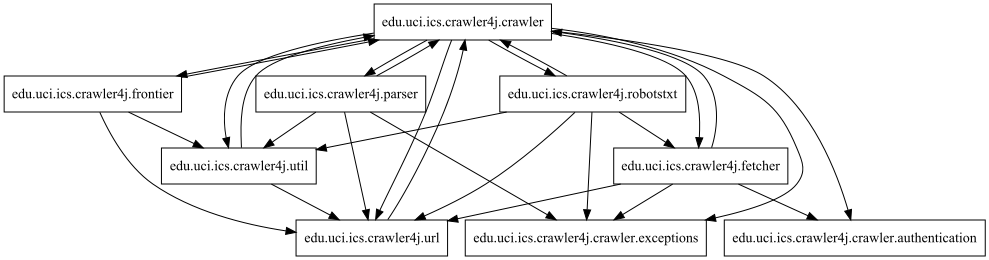
\includegraphics[scale=0.4]{img/crawler_packages_orig}
    \caption{\textit{crawler4j} sistemos struktūra}
    \label{fig:crawler_packages_orig}
\end{figure}

Atlikus sistemos kokybės matų analizę, gautą rezultatą galima naudoti problemų paieškai sistemoje (pavyzdys~\ref{table:crawlers}).
\begin{figure}[H]
\begin{center}
    \begin{tabular}{|c|c|c|c|c|c|c|c|}
        \hline
        Paketo vardas & \textit{N} & \textit{A} & \textit{E} & \textit{S} & \textit{A} & \textit{D} & \textit{C} \\ [0.5ex]
        \hline\hline
        edu.uci.ics.crawler4j.crawler.authentication & 4 & 2 & 0 & 0.0 & 0.25 & 0.75 & 0\\
        \hline
        edu.uci.ics.crawler4j.url & 4 & 6 & 1 & 0.143 & 0.0 & 0.857 & 1 \\
        \hline
        edu.uci.ics.crawler4j.crawler.exceptions & 3 & 4 & 0 & 0.0 & 0.0 & 1.0 & 0\\
        \hline
        edu.uci.ics.crawler4j.crawler & 5 & 6 & 8 & 0.571 & 0.2 & 0.229 & 5 \\
        \hline
        edu.uci.ics.crawler4j.robotstxt & 6 & 1 & 5 & 0.833 & 0.0 & 0.167 & 1 \\
        \hline
        edu.uci.ics.crawler4j.frontier & 6 & 1 & 3 & 0.75 & 0.0 & 0.25 & 1 \\
        \hline
        edu.uci.ics.crawler4j.fetcher & 6 & 2 & 4 & 0.667 & 0.0 & 0.333 & 1 \\
        \hline
        edu.uci.ics.crawler4j.util & 3 & 4 & 2 & 0.333 & 0.0 & 0.667 & 0 \\
        \hline
        edu.uci.ics.crawler4j.parser & 12 & 1 & 4 & 0.8 & 0.167 & 0.033 & 1 \\
        \hline
    \end{tabular}
    \begin{tabular}{|c|c|c|c|c|c|c|c|}
        \hline
        Vidurkiai & $\bar{N}$ & $\bar{Af}$ & $\bar{Ef}$ & $\bar{S}$ & $\bar{A}$ & $\bar{D}$ & $\Sigma C$  \\ [0.5ex]
        \hline\hline
        & 5 & 3 & 3 & 0.455 & 0.069 & 0.476 & 5\\
        \hline
    \end{tabular}
\end{center}
\caption{\textit{crawler4j} paketų kokybės matai}
\label{table:crawlers}
\end{figure}
\textbf{Matų lentelės paaiškinimas}:
\begin{itemize}
    \item \textit{N} - klasių skaičių pakete.
    \item \textit{Af} - aferentinės jungtys.
    \item \textit{Ef} - eferentinės jungtys.
    \item \textit{S} - stabilumas.
    \item \textit{A} - paketo abstraktuma.
    \item \textit{D} - atstumas nuo pagrindinės sekos.
    \item \textit{C} - ciklinių priklausomybių skaičius.
\end{itemize}
Kaip skaičiuojami matai aprašyta paketų kokybės matų skyriuje~\ref{sec:matai}, puslapyje~\pageref{sec:matai}.

Iš bendros sistemos analizės bei matų lentelės rezultatų matomos kelios sistemos problemos -
\begin{itemize}
    \item \textbf{Problema numeris 1} - atlikus bendrą sistemos kodo analizę matoma,
    kad sistemos paketuose yra sąsajos, kurios turi daugiau nei vieną įgyvendinimą, neturint šablono, nusakančio, kaip skirstyti skirtingus įgyvendinimus pasidaro sudėtinga
    rasti tinkamą specifinės sąsajos įgyvendinimą.
    \item \textbf{Problema numeris 2} - paketo \textit{edu.uci.ics.crawler4j.parser} viduje yra 12 klasių, turinčių skirtingas atsakomybes, todėl yra sunku suprasti,
    kokią funkciją atlieka šis paketas, kokie pokyčiai produkte gali pareikalauti jo pakeitimų.
    \item \textbf{Problema numeris 3} - sistema turi daug ciklinių prilausomynbių, kur du arba daugiau paketų priklauso vienas nuo kito.
    Tai matoma sistemos paketų diagramoje pavyzdyje~\ref{fig:crawler_packages_orig}, ciklinėse priklausomybėse dalyvauja 10 paketų ir kartu jie sudaro 5 ciklinių priklausomybių sekas,
    kurios turėtų būti pašalintos.
\end{itemize}

Sistemos paketas \textit{edu.uci.ics.crawler4j.parse}, turi sąsają \textit{ParseData} bei 4 skirtingus jos įgyvendinimus - \textit{CssParseData, TextParseData, HtmlParseData, BinaryParseData},
šios klasės pakete dalinasi vieta dar su 9 klasėmis, todėl yra nepatogu rasti ieškomą įgyvendinimą (pavyzdys~\ref{fig:parse}).
\begin{figure}[H]
    \snugshade
    \dirtree{%
        .1 {/parser} .
        .2 {AllTagMapper}.
        .2 {ParseData}.
        .2 {TextParseData}.
        .2 {HtmlParseData}.
        .2 {CssParseData}.
        .2 {BinaryParseData}.
        .2 {ExtractedUrlAnchorPair}.
        .2 {HtmlParser}.
        .2 {HtmlContentHandler}.
        .2 {TikaHtmlParser}.
        .2 {Parser}.
    }
    \endsnugshade
    \caption{\textit{parser} paketo struktūra}
    \label{fig:parse}
\end{figure}
Šiam paketui sutvarkyti taikomas \textit{įgyvendinimų atskyrimo} šablonas - sąsaja iškeliama į atskirą paketą \textit{parse}, jos įgyvendinimai perkeliami į minėto
paketo subpaketus.
Šie pertvarkymai pakeičia \textit{parser} paketo struktūrą (pavyzdys~\ref{fig:parser}).
\begin{figure}[H]
    \snugshade
    \dirtree{%
        .1 {/parser} .
        .2 {parse}.
        .3 {ParseData // Sąsaja}.
        .3 {text}.
        .4 {TextParseData // Pirmas sąsajos įgyvendinimas}.
        .3 {html }.
        .4 {HtmlParseData // Antras sąsajos įgyvendinimas}.
        .3 {css }.
        .4 {CssParseData // Trečias sąsajos įgyvendinimas}.
        .3 {binary}.
        .4 {BinaryParseData // Ketvirtas sąsajos įgyvendinimas}.
        .2 {AllTagMapper}.
        .2 {ExtractedUrlAnchorPair}.
        .2 {HtmlParser}.
        .2 {HtmlContentHandler}.
        .2 {NotAllowedContentException}.
        .2 {TikaHtmlParser}.
        .2 {Parser}.
    }
    \endsnugshade
    \caption{\textit{parser} paketo struktūra po pirmojo pertvarkymo}
    \label{fig:parser}
\end{figure}
Dėl atskirtos sąsajos ir jos įgyvendinimų tampa paprasčiau ją rasti bei suprasti sistemoje egzistuojančius jos įgyvendinimus.
Tokia struktūra išsprendžia sistemos \textbf{problemą numeris 1}.
Šis pertvarkymas taip pat dalinai sumažino \textbf{problemą numeris 2}, sumažinant klasių skaičių pakete į 7.
Palyginus pertvarkytos ir buvusios sistemos matus matome, kad sistema tapo aiškesnė - sumažėjo vidutinis klasių skaičius paketuose,
todėl yra paprasčiau suprasti pagrindines paketų funkcijas.
Nors nežymiai sumažėjo vidutinis stabilumas, bet pakilo abstrakcijos lygis, todėl atstumas nuo pagrindinės sekos sumažėjo (pavyzdys~\ref{table:parsers}).
\begin{figure}[H]
\begin{center}
    \begin{tabular}{|c|c|c|c|c|c|c|c|}
        \hline
        \textit{crawler4j.parser} & \textit{N} & \textit{A} & \textit{E} & \textit{S} & \textit{A} & \textit{D} & \textit{C} \\ [0.5ex]
        \hline\hline
        Prieš & 12 & 1 & 4 & 0.8 & 0.167 & 0.033 & 1 \\
        \hline
        Po & \cellcolor{green!25} 7 (-5) & 1 & 9 & \cellcolor{red!25} 0.9 + (0.1) & \cellcolor{red!25} 0.143 (-0.024) & \cellcolor{red!25} 0.043 (+0.01) & 1 \\
        \hline
    \end{tabular}
    \begin{tabular}{|c|c|c|c|c|c|c|c|}
        \hline
        Vidurkiai & $\bar{N}$ & $\bar{Af}$ & $\bar{Ef}$ & $\bar{S}$ & $\bar{A}$ & $\bar{D}$ & $\Sigma C$ \\ [0.5ex]
        \hline\hline
        Prieš & 5 & 3 & 3 & 0.455 & 0.069 & 0.476 & 5\\
        \hline
        Po & \cellcolor{green!25} 4 (-1) & 3 & 3 & \cellcolor{red!25} 0.488 (+0.033) & \cellcolor{green!25} 0.114 (+0.045) & \cellcolor{green!25} 0.425 (-0.051) & 5 \\
        \hline
    \end{tabular}
\end{center}
\caption{\textit{crawler4j} paketų kokybės matai po pirmo pertvarkymo}
\label{table:parsers}
\end{figure}
Matų įverčio didėjimas nebūtinai susijęs su sistemos kokybės gerėjimu, todėl teigiamas pokytis paženklintas žaliai, o neigiamas - raudonai.
Norint išspręsti \textbf{problemą numeris 3} - ciklines priklausomybes, reikia identifikuoti klases, kurių priklausomybės
sudaro ciklus ir iškelti jas į atskirus paketus.

Kuriant naujus paketus vadovaujamasi \textit{skirstymo pagal smulkų funkcionalumą} šablonu, užtikrinant, kad kiekvienas
paketas teikia vieną, aiškiai apibrėžtą funkciją, kuri yra pasiekiama per pakete aprašytą sąsają.
Paketo vidus yra paslėptas su \textit{Java} kalbos pasiekiamumo modifikatoriais - konkrečių klasių negalima inicializuoti arba paveldėti už paketo ribų,
nes jų konstruktoriai privatūs (pavyzdys~\ref{fig:sasaja}). Klasės inicializuojamos statinių metodų pagalba, kurie grąžina inicializuotas konkrečias klases, įgyvendinančias reikiamą
sąsają.

\begin{figure}[H]
    \begin{lstlisting}[language=Python]
public interface HtmlParser {

    HtmlParseData parse(ParsedPage page, String contextURL) throws ParseException;

    // Grazinamas sasajos igyvendinimas
    static HtmlParser newHtmlParser(CrawlConfig config, TLDList tldList) throws InstantiationException, IllegalAccessException {
        return new TikaHtmlParser(config, tldList);
    }
}

// Sasajos igyvendinimas. Nera viesas, pasiekiamas tik paketo viduje, nes klase ir konstruktorius nenaudoja public raktazodziu
class TikaHtmlParser implements HtmlParser {
   ...
    TikaHtmlParser(CrawlConfig config, TLDList tldList) throws InstantiationException, IllegalAccessException {
     ...
    }
    \end{lstlisting}
    \caption{Sąsaja parašyta laikantis \textit{skirstymo pagal teikiamą funkcionalumą} šablono gairių}
    \label{fig:sasaja}
\end{figure}
Peržiūrėjus paketus su ciklinėmis priklausomybėmis, iš jų buvo išskirti šie nauji funkcionalumai, kuriems
buvo sukurti atskiri paketai (pavyzdys~\ref{fig:crawlerj},~\ref{fig:crawlerjs}).
\begin{itemize}
    \item Iš \textit{parser} paketo iškeltas funkcionalumas \textit{html} turiniui apdoroti, patalpintas į \textit{parser/html} paketą.
    Po šio pertvarkymo \textit{parser} paketas pasidaro mažesnis ir turi vieną funkcionalumą - priimti puslapį ir deleguoti jį apdorojimui kitai klasei pagal puslapio tipą.
    \item Iš \textit{robotstxt} paketo funkcionalumas patikrinti, ar sistema autorizuota apdoroti pasirinktą puslapį, iškeltas į \textit{robotstxt/permissions} paketą.
    \item Iš \textit{crawler}, bei \textit{parser} paketų funkcionalumas, aprašantis internetinio puslapio elementus, iškeltas į \textit{web} paketą.
    \item Iš \textit{crawler} paketo funkcionalumas, nustatantis įrankio konfigūraciją, iškeltas į \textit{config} paketą.
    \item Iš \textit{url} paketo funkcionalumas, gaunantis internetinių domenų pavadinimus, iškeltas į \textit{tld} paketą.
\end{itemize}

\begin{figure}[H]
    \snugshade
    \dirtree{%
        .1 {/} .
        .2 {crawler4j}.
        .3 {crawler}.
        .4 {authentication}.
        .4 {exceptions}.
        .3 {fetcher}.
        .3 {frontier}.
        .3 {parser}.
        .4 {parse}.
        .5 {binary}.
        .5 {css}.
        .5 {factory}.
        .5 {html}.
        .5 {text}.
        .3 {robotstxt}.
        .3 {url}.
        .3 {util}.
    }
    \endsnugshade
    \caption{\textit{crawler4j} paketų medis prieš iškeliant minėtus funkcionalumus}
    \label{fig:crawlerj}
\end{figure}

\begin{figure}[H]
    \snugshade
    \dirtree{%
        .1 {/} .
        .2 {crawler4j}.
        .3 {config}.
        .3 {crawler}.
        .4 {authentication}.
        .3 {fetcher}.
        .3 {frontier}.
        .3 {parser}.
        .4 {html}.
        .4 {parse}.
        .5 {binary}.
        .5 {css}.
        .5 {html}.
        .5 {text}.
        .3 {robotstxt}.
        .4 {permissions}.
        .3 {tld}.
        .3 {util}.
        .3 {web}.
    }
    \endsnugshade
    \caption{\textit{crawler4j} paketų medis iškėlus minėtus funkcionalumus}
    \label{fig:crawlerjs}
\end{figure}

Atlikus šiuos funkcionalumų suskaidymus į atskirus paketus buvo panaikintos žiedinės priklausomybės.
Naujoje paketų diagramoje galime matyti, jog dabar sistema turi daugiau paketų, tačiau jų priklausomybių kryptys yra aiškesnės (pavyzdys~\ref{img:crawler_packages_v2}).
\begin{figure}[H]
    \centering
    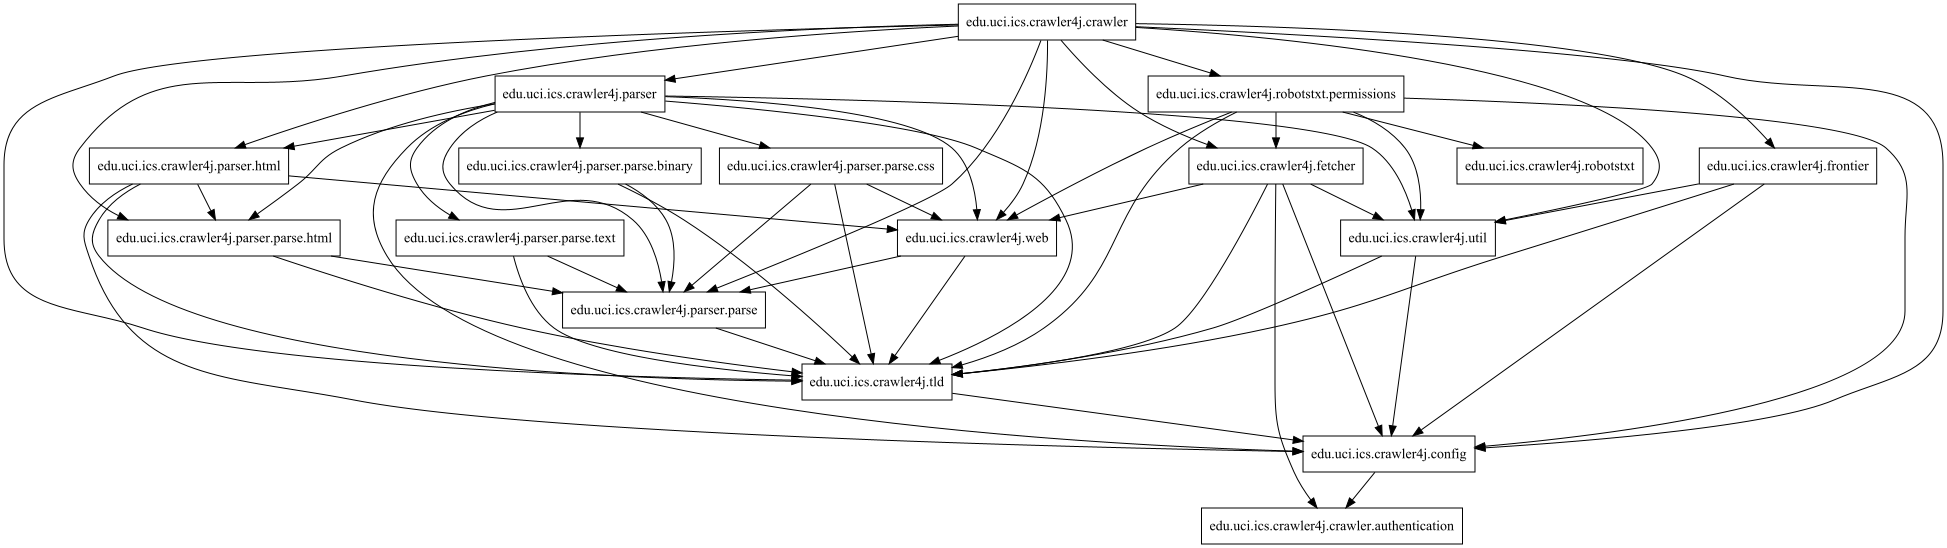
\includegraphics[scale=0.22]{img/crawler_packages_v2}
    \caption{\textit{crawler4j} sistemos struktūra po antro pertvarkymo}
    \label{img:crawler_packages_v2}
\end{figure}

Atlikus matų analizę pertvarkytai sistemai yra matoma, kad sistemos kokybė pagerėjo:
sumažėjo vidutinis klasių skaičius pakete, ciklinių priklausomybių rodiklis tapo lygus nuliui,
padidėjo vidutinis abstrakcijos lygis (pavyzdys~\ref{table:abstrs}).
\begin{figure}[H]
\begin{center}
    \begin{tabular}{|c|c|c|c|c|c|c|c|}
        \hline
        Paketo vardas & \textit{N} & \textit{Af} & \textit{Ef} & \textit{S} & \textit{A} & \textit{D} & \textit{C} \\ [0.5ex]
        \hline\hline
        edu.uci.ics.crawler4j.parser.parse.binary & 1 & 1 & 2 & 0.667 & 0.0 & 0.333 & 0 \\
        \hline
        edu.uci.ics.crawler4j.crawler & 4 & 0 & 11 & 1.0 & 0.25 & 0.25 & 0 \\
        \hline
        edu.uci.ics.crawler4j.tld & 3 & 13 & 1 & 0.071 & 0.333 & 0.596 & 0 \\
        \hline
        edu.uci.ics.crawler4j.parser.html & 6 & 2 & 4 & 0.667 & 0.167 & 0.166 & 0 \\
        \hline
        edu.uci.ics.crawler4j.robotstxt.permissions & 2 & 1 & 6 & 0.857 & 0.5 & 0.357 & 0 \\
        \hline
        edu.uci.ics.crawler4j.config & 1 & 8 & 1 & 0.111 & 0.0 & 0.889 & 0 \\
        \hline
        edu.uci.ics.crawler4j.frontier & 6 & 1 & 3 & 0.75 & 0.0 & 0.25 & 0 \\
        \hline
        edu.uci.ics.crawler4j.parser & 2 & 1 & 10 & 0.909 & 0.0 & 0.091 & 0\\
        \hline
        edu.uci.ics.crawler4j.crawler.authentication & 4 & 2 & 0 & 0.0 & 0.25 & 0.75 & 0 \\
        \hline
        edu.uci.ics.crawler4j.parser.parse.css & 1 & 1 & 3 & 0.75 & 0.0 & 0.25 & 0 \\
        \hline
        edu.uci.ics.crawler4j.robotstxt & 5 & 1 & 0 & 0.0 & 0.0 & 1.0 & 0 \\
        \hline
        edu.uci.ics.crawler4j.parser.parse.html & 1 & 3 & 2 & 0.4 & 0.0 & 0.6 & 0 \\
        \hline
        edu.uci.ics.crawler4j.parser.parse & 1 & 7 & 1 & 0.125 & 1.0 & 0.125 & 0\\
        \hline
        edu.uci.ics.crawler4j.fetcher & 6 & 2 & 5 & 0.714 & 0.0 & 0.286 & 0 \\
        \hline
        edu.uci.ics.crawler4j.util & 4 & 5 & 2 & 0.286 & 0.0 & 0.714 & 0 \\
        \hline
        edu.uci.ics.crawler4j.web & 5 & 6 & 2 & 0.25 & 0.4 & 0.35 & 0 \\
        \hline
        edu.uci.ics.crawler4j.parser.parse.text & 1 & 1 & 2 & 0.667 & 0.0 & 0.333 & 0 \\
        \hline
    \end{tabular}
    \begin{tabular}{|c|c|c|c|c|c|c|c|}
        \hline
        Vidurkiai & $\bar{N}$ & $\bar{Af}$ & $\bar{Ef}$ & $\bar{S}$ & $\bar{A}$ & $\bar{D}$ & $\Sigma C$ \\ [0.5ex]
        \hline\hline
        Pradiniai & 5 & 3 & 3 & 0.455 & 0.069 & 0.476 & 5\\
        \hline
        Po & \cellcolor{green!25} 3 (-2) & 3 & 3 & \cellcolor{green!24} 0.452 (-0.03) & \cellcolor{green!25} 0.183 (+0.114) & \cellcolor{green!25} 0.471 (-0.005) & \cellcolor{green!25} 0 (-5)\\
        \hline
    \end{tabular}
\end{center}
\caption{\textit{crawler4j} paketų kokybės matai po galutinių pertvarkymų}
\label{table:abstrs}
\end{figure}
Iš gautų rezultatų galime teigti, jog po pertvarkymo šablonai \textit{skirstymas pagal smulkų funkcionalumą} ir \textit{įgyvendinimų atskyrimas}, išsprendė visas 3 sistemoje matytas problemas,
padarė sistemą lengviau suprantama, panaikino ciklines priklausomybes ir turėjo teigiamą įtaką matams, nurodantiems
sistemos įgyvendinimo kokybę.


\subsection{\textit{azure-sdk-for-java} sistema}
\textbf{azure-sdk-for-java\footnote{\url{https://github.com/Azure/azure-sdk-for-java/tree/main/sdk/storage/azure-storage-blob-cryptography}}} yra atviro kodo
biblioteka, parašyta \textit{Java} programavimo kalba, leidžianti programiškai bendrauti su \textit{Microsoft Azure} debesų kompiuterijos platforma.
Tai programinės įrangos įrankis, skirtas naudoti kitose sistemose, supaprastinant programinį kodą.
Ši biblioteka yra labai didelė ir šio pertvarkymo metu yra dirbama tik su posisteme \textit{azure-storage-blob-cryptograph} kuri atsakinga už duomenų kriptografiją
komunikacijos su \textit{Azure Blob} nestruktūrizuota failų saugykla metu.

Prieš visus pakeitimus \textit{azure-storage-blob-cryptograph} sistema turi vieną paketą \textit{com.azure.storage.blob.specialized.cryptography}, kuriame guli visos jos klasės.

Sistemos kokybės matai nėra naudingi dirbant su vienu paketu, nes trūksta konteksto suprasti, kaip paketas yra naudojamas.
Tačiau iš bendrinės sistemos analizės galima pamatyti pagrindines sistemos problemas - viename pakete yra 21 skirtinga klasė - tiek sąsajos, tiek konkrečios klasės.
Taip pat sistemoje yra kelios skirtingos tos pačios esybės versijos - \textit{DecryptorV1} ir \textit{DecryptorV2}, \textit{EncryptorV1} ir \textit{EncryptorV2}, todėl sunku
suprasti, su kokia esybės versija yra susijusios kitos klasės bei yra kodo pasikartojimo.
Ši sistema būtų aiškesnė ir greičiau perprantama, jei būtų išskirti mažesni funkcionalumai ir kodas būtų išskaidytas į smulkesnius paketus, taip pat atskiriant juos
pagal esybių versijas.
Norint atlikti esybių versijavimą naudojamas \textit{skirtingų versijų grupavimo į paketus} šablonas, pagal jį kiekvienai esybės versijai sukuriamas atskiras paketas,
taip pat bendras, pasikartojantis kodas iškeliamas į abstrakčią klasę, kuri yra pakete vienu lygiu aukščiau nei versijų paketai (pokyčių pavyzdžiai ~\ref{fig:rep1}, ~\ref{fig:rep2}).

\begin{figure}[H]
    \snugshade
    \dirtree{%
        .1 {/cryptography} .
        .2 {Decryptor} .
        .2 {DecryptorV1 // Pirma esybės versija} .
        .2 {DecryptorV2 // Antra esybės versija} .
        .2 {Encryptor} .
        .2 {EncryptorV1 // Pirma esybės versija} .
        .2 {EncryptorV2 // Antra esybės versija} .
        .2 {\ldots // Likusios klasės lieka pagrindiniame pakete} .
    }
    \endsnugshade
    \caption{\textit{azure-storage-blob-cryptograph} kriptografijos klasių struktūra prieš pertvarkymą}
    \label{fig:rep1}
\end{figure}

\begin{figure}[H]
    \snugshade
        \dirtree{%
            .1 {/cryptography} .
            .2 {decryptor} .
            .3 {Decryptor // Abstrakti klasė su bendru esybės kodu} .
            .3 {v1} .
            .4 {DecryptorV1 // Pirma esybės versija} .
            .3 {v2} .
            .4 {DecryptorV2 // Antra esybės versija} .
            .2 {encryptor} .
            .3 {Encryptor // Abstrakti klasė su bendru esybės kodu} .
            .3 {agent // Papildomas, su esybe susijęs kodas, naudojamas abiejų esybių} .
            .3 {v1} .
            .4 {EncryptorV1 // Pirma esybės versija} .
            .3 {v2} .
            .4 {EncryptorV2 // Antra esybės versija} .
            .2 {\ldots // Likusios klasės lieka pagrindiniame pakete} .
        }
    \endsnugshade
    \caption{\textit{azure-storage-blob-cryptograph} kriptografijos klasių struktūra po jų iškėlimo į paketus}
    \label{fig:rep2}
\end{figure}
Šis pertvarkymas pagal \textit{skirtingų versijų grupavimo į paketus} šabloną, atskiria esybės versijas ir sukuria naujus paketus, apibrėžiančius aiškesnius funkcionalumus.
Atsiradus daugiau paketų bei jų sąsajų, galima paskaičiuoti paketų kokybės matus:
\begin{figure}[H]
\begin{center}
    \begin{tabular}{|c|c|c|c|c|c|c|c|}
        \hline
        Paketo vardas & \textit{N} & \textit{Af} & \textit{Ef} & \textit{S} & \textit{A} & \textit{D} & \textit{C} \\ [0.5ex]
        \hline\hline
        specialized.cryptography & 13 & 7 & 5 & 0.417 & 0.0 & 0.583 & 5 \\
        \hline
        specialized.cryptography.encryptor.v2 & 1 & 1 & 3 & 0.75 & 0.0 & 0.25 & 0 \\
        \hline
        specialized.cryptography.encryptor.v1 & 1 & 0 & 3 & 1.0 & 0.0 & 0.0 & 1 \\
        \hline
        specialized.cryptography.encryptor & 1 & 4 & 2 & 0.333 & 1.0 & 0.333 & 2 \\
        \hline
        specialized.cryptography.decryptor.v2 & 1 & 1 & 2 & 0.667 & 0.0 & 0.333 & 1 \\
        \hline
        specialized.cryptography.decryptor.v1 & 1 & 1 & 2 & 0.667 & 0.0 & 0.333 & 1\\
        \hline
        specialized.cryptography.encryptor.agent & 2 & 3 & 2 & 0.4 & 0.0 & 0.6 & 1\\
        \hline
        specialized.cryptography.decryptor & 2 & 3 & 1 & 0.25 & 0.5 & 0.25 & 1 \\
        \hline
    \end{tabular}
    \begin{tabular}{|c|c|c|c|c|c|c|c|}
        \hline
        Vidurkiai & $\bar{N}$ & $\bar{Ag}$ & $\bar{Eg}$ & $\bar{S}$ & $\bar{A}$ & $\bar{D}$ & $\Sigma C$ \\ [0.5ex]
        \hline\hline
        & 3 & 3 & 3 & 0.561 & 0.188 & 0.335 & 6 \\
        \hline
    \end{tabular}
\end{center}
\caption{\textit{azure-storage-blob-cryptograph} paketų kokybės matai po pirmo pertvarkymo}
\label{table:matais}
\end{figure}
Apskaičiuoti matai (pavyzdys~\ref{table:matais}) rodo nedidelį nuokrypį nuo pagrindinės sekos, todėl galima teigti, kad sistemos abstraktumas bei stabilumas
yra subalansuoti, tačiau šis skirstymas turėjo ir neigiamų padarinių - sukelė 6 ciklines priklausomybes.
Šiais priklausomybes galima matyti sistemos paketų diagramoje (pavyzdys~\ref{fig:azure_packages_v1}).
\begin{figure}[H]
    \centering
    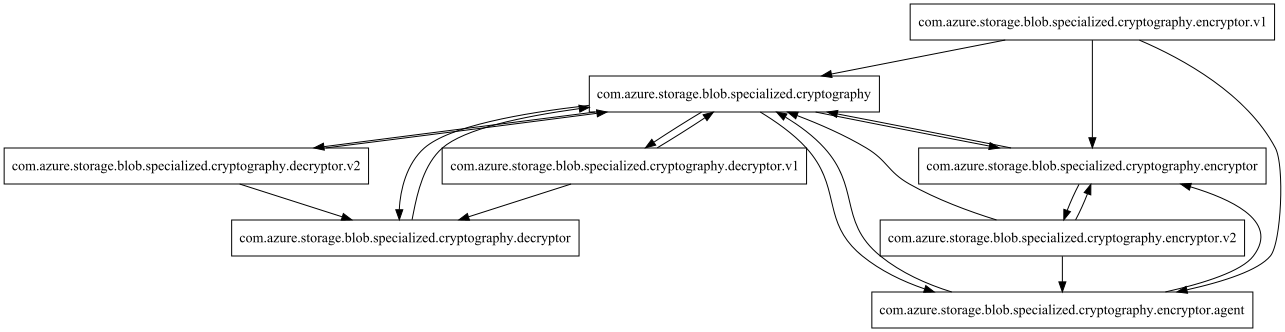
\includegraphics[scale=0.35]{img/azure_packages_v1}
    \caption{\textit{azure-storage-blob-cryptograph} sistemos struktūra po pirmojo pertvarkymo}
    \label{fig:azure_packages_v1}
\end{figure}
Norint panaikinti ciklines priklausomybes, reikia panaudoti \textit{skirstymo pagal smulkų funkcionalumą} šabloną ir, išskaidant pagrindinį paketą
į dar smulkesnius vienetus - yra sukuriamas \textit{encryption.data} paketas, atsakingas už užkoduotų duomenų vaizdavimą, taip pat
aprašomas paketas \textit{blob} skirtas \textit{blob} esybių, reprezentuojančių saugyklos duomenų formatą, kriptografijai.
Taip pat vadovaujantis \textit{atskiro pagalbinių klasių paketo} šablonu, visos pagalbinės klasės, neturinčios priklausomybių į kitus paketus ir
padedančios vykdyti kertinius techninius funkcionalumus yra iškeliamos į \textit{util} paketą.
Minėtame pakete atsiranda tokios klasės:
\begin{itemize}
    \item \textit{CryptographyConstants} - klasė, saugojanti bendras, su kriptografija susijusias konstantas, kurios naudojamos skirtingose sistemos vietose.
    \item \textit{EncryptionVersion} - aprašo kriptografijos versijas ir jų naudojamus protokolus
    \item \textit{WrappedKeyJson} - palengvina darbą serializuojant ir deserializuojant kriptografijos raktus į \textit{json} formatą.
\end{itemize}

Pritaikius visus šiuos šablonus, gaunama sistemos struktūra turinti nedidelius, aiškesniais funkcionalumais apibrėžtus paketus,
taip pat pašalinamos ciklinės priklausomybės (pavyzdys~\ref{fig:azure_packages_v2}).
\begin{figure}[H]
    \centering
    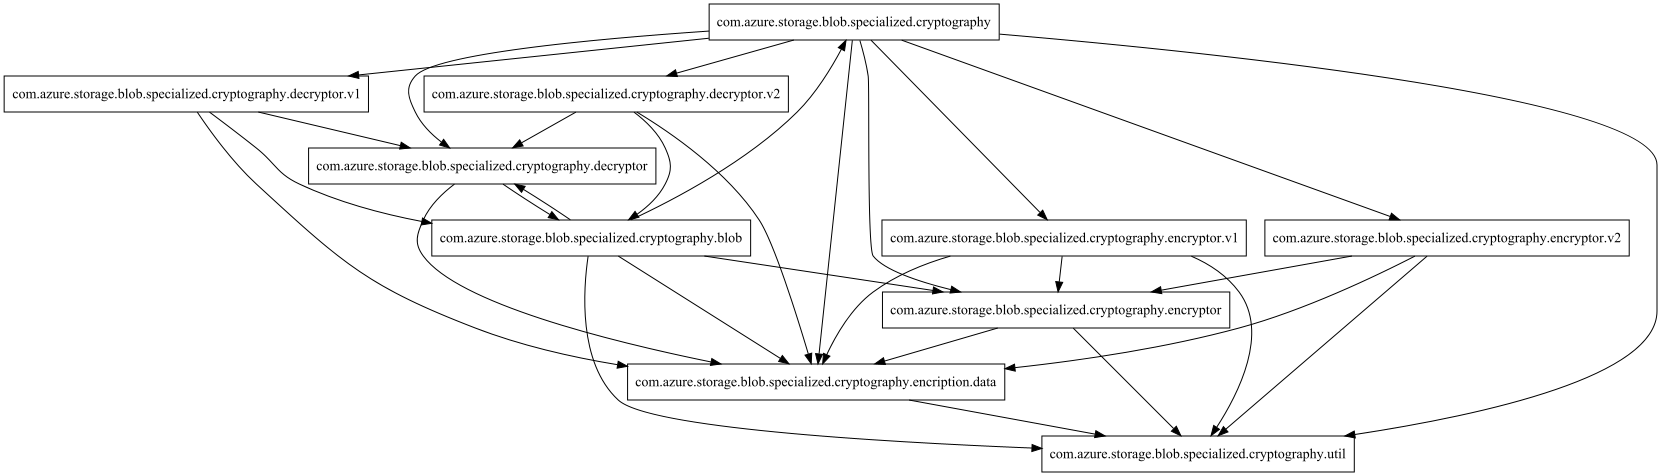
\includegraphics[scale=0.27]{img/azure_packages_v2}
    \caption{Galutinė \textit{azure-storage-blob-cryptograph} sistemos struktūra}
    \label{fig:azure_packages_v2}
\end{figure}

Pakartotinai įvertinus matus matoma, kad nuokrypis nuo pagrindinės sekos šiek tiek padidėjo, tačiau
vis dar yra gan mažas, ciklinės priklausomybės išnyko, todėl galime teigti, kad \textit{skirstymo pagal smulkų funkcionalumą},
\textit{atskiro pagalbinių klasių paketo} ir \textit{skirtingų versijų grupavimo į paketus} šablonai prisidėjo prie bendro
sistemos suprantamumo, įvedė aiškesnę jos struktūrą, nesukuriant sistemos kokybės problemų, aptinkamų paketų kokybės matuose (pavyzdys~\ref{table:verts}).
\begin{figure}[H]
\begin{center}
    \begin{tabular}{|c|c|c|c|c|c|c|c|}
        \hline
        Paketo vardas & \textit{N} & \textit{Af} & \textit{Ef} & \textit{S} & \textit{A} & \textit{D} & \textit{C} \\ [0.5ex]
        \hline\hline
        specialized.cryptography & 3 & 1 & 8 & 0.889 & 0.0 & 0.111 & 0 \\
        \hline
        specialized.cryptography.blob & 6 & 3 & 5 & 0.625 & 0.0 & 0.375 & 0 \\
        \hline
        specialized.cryptography.encription.data & 4 & 8 & 1 & 0.111 & 0.0 & 0.889 & 0 \\
        \hline
        specialized.cryptography.encryptor.v2 & 1 & 1 & 3 & 0.75 & 0.0 & 0.25 & 0 \\
        \hline
        specialized.cryptography.encryptor.v1 & 1 & 1 & 3 & 0.75 & 0.0 & 0.25 & 0 \\
        \hline
        specialized.cryptography.encryptor & 1 & 4 & 2 & 0.333 & 1.0 & 0.333 & 0 \\
        \hline
        specialized.cryptography.decryptor.v2 & 1 & 1 & 3 & 0.75 & 0.0 & 0.25 & 0 \\
        \hline
        specialized.cryptography.decryptor.v1 & 1 & 1 & 3 & 0.75 & 0.0 & 0.25 & 0 \\
        \hline
        specialized.cryptography.decryptor & 2 & 4 & 2 & 0.333 & 0.5 & 0.167 & 0 \\
        \hline
        specialized.cryptography.util & 3 & 6 & 0 & 0.0 & 0.0 & 1.0 & 0 \\
        \hline
    \end{tabular}
    \begin{tabular}{|c|c|c|c|c|c|c|c|}
        \hline
        Vidurkiai & $\bar{N}$ & $\bar{A}$ & $\bar{E}$ & $\bar{S}$ & $\bar{A}$ & $\bar{D}$ & $\Sigma C$ \\ [0.5ex]
        \hline\hline
        Pertvarkymas 1 & 3 & 3 & 3 & 0.561 & 0.188 & 0.335 & 6 \\
        Pertvarkymas 2 & \cellcolor{green!25} 2 (-1) & 3 & 3 & \cellcolor{green!25} 0.529 (-0.032) & \cellcolor{red!25} 0.15 (-0.03) & \cellcolor{red!25} 0.388 (+0.053) &  \cellcolor{green!25} 0 (-5) \\
        \hline
    \end{tabular}
\end{center}
\caption{\textit{azure-storage-blob-cryptograph} paketų kokybės matai po visų pertvarkymų}
\label{table:verts}
\end{figure}


Pavyzdyje~\ref{table:sistemos} matomos pertvarkytos sistemos, jose rastos problemos ir šablonų, panaudotų problemų išsprendimui, sąrašas.
Pertvarkytų sistemų programinis kodas yra pasiekiamas viešoje \textit{GitHub}\footnote{\url{https://github.com/MartynaUb/bachelor-thesis-analysis-of-code-packaging-patterns/tree/main/code/refactored_systems}} repozitorijoje.
\begin{figure}[H]
    \begin{tabular}{|p{3cm}|p{6cm}|p{6cm}|}
        \hline
        Sistema                                                                                           & Išspręstos problemos                                                                                                   & Panaudoti šablonai                                                                                    \\ \hline\hline
        crawler4j                        & Dideli paketai su skirtingomis atsakomybėmis, neaiški struktūra sąsajos įgyvendimams saugoti, ciklinės priklausomybės & Skirstymas pagal smulkų funkcionalumą, įgyvendinimų atskyrimas                                        \\ \hline
        azure storage blob cryptography  & Dideli paketai su skirtingomis atsakomybėmis, nėra pagalbinių klasių paketų, skirtingos tos pačios esybės versijos    & Skirstymas pagal smulkų funkcionalumą, atskirų versijų skirstymas, atskiras pagalbinių klasių paketas \\ \hline
    \end{tabular}
    \caption{Pertvarkytos sistemos ir panaudoti šablonai}
    \label{table:sistemos}
\end{figure}

Atlikus sistemų pertvarkymus buvo gauti matų rezultatai, įrodantys, jog atrinkti šablonai prisideda ne tik prie kodo suprantamumo žmogui, bet ir daro
teigiamą įtaką sistemos kokybei - daugumoje atvejų mažina ciklines priklausomybes, vidutinį klasių skaičių pakete, atstumą nuo pagrindinės sekos.

\sectionnonum{Rezultatai}
Rezultatų skyriuje išdėstomi pagrindiniai darbo rezultatai: kažkas išanalizuota,
kažkas sukurta, kažkas įdiegta. Tarpinių žingsnių išdavos skirtos užtikrinti galutinio
rezultato kokybę neturi būti pateikiami šiame skyriuje. Kalbant informatikos termi-
nais, šiame skyriuje pateikiama darbo išvestis, kuri gali būti įvestimi kituose panašios
tematikos darbuose. Rezultatai pateikiami sunumeruotų (gali būti hierarchiniai) sąrašų
pavidalu. Darbo rezultatai turi atitikti darbo tikslą.

\sectionnonum{Išvados}
\begin{enumerate}[labelindent=0pt]
    \item Išvadų skyriuje daromi nagrinėtų problemų sprendimo metodų palyginimai, siūlomos
rekomendacijos, akcentuojamos naujovės.
    \item Išvados pateikiamos sunumeruoto (gali būti hierarchinis) sąrašo pavidalu.
    \item Darbo išvados turi atitikti darbo tikslą.
\end{enumerate}

\printbibliography[heading=bibintoc]  % Šaltinių sąraše nurodoma panaudota
% literatūra, kitokie šaltiniai. Abėcėlės tvarka išdėstomi darbe panaudotų
% (cituotų, perfrazuotų ar bent paminėtų) mokslo leidinių, kitokių publikacijų
% bibliografiniai aprašai. Šaltinių sąrašas spausdinamas iš naujo puslapio.
% Aprašai pateikiami netransliteruoti. Šaltinių sąraše negali būti tokių
% šaltinių, kurie nebuvo paminėti tekste (LaTeX tai sutvarko automatiškai).
% Šaltinių sąraše rekomenduojame necituoti savo kursinio darbo, nes tai nėra
% oficialus literatūros šaltinis. Jei tokių nuorodų reikia, pateikti jas tekste.

% Priedai
% Prieduose gali būti pateikiama pagalbinė, ypač darbo autoriaus savarankiškai
% parengta, medžiaga. Savarankiški priedai gali būti pateikiami ir
% kompaktiniame diske. Priedai taip pat numeruojami ir vadinami. Darbo tekstas
% su priedais susiejamas nuorodomis.
%\appendix{Neuroninio tinklo struktūra}
%
%\begin{figure}[H]
%    \centering
%    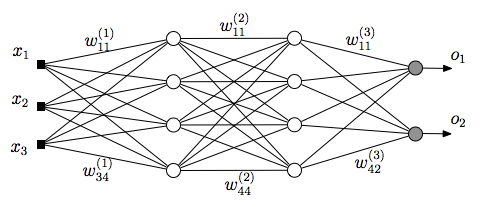
\includegraphics[scale=0.5]{img/MLP}
%    \caption{Paveikslėlio pavyzdys}
%    \label{img:mlp}
%\end{figure}


%\appendix{Eksperimentinio palyginimo rezultatai}
%
%% tablesgenerator.com - converts calculators (e.g. excel) tables to LaTeX
%\begin{table}[H]\footnotesize
%  \centering
%  \caption{Lentelės pavyzdys}
%  {\begin{tabular}{|l|c|c|} \hline
%    Algoritmas & $\bar{x}$ & $\sigma^{2}$ \\
%    \hline
%    Algoritmas A  & 1.6335    & 0.5584       \\
%    Algoritmas B  & 1.7395    & 0.5647       \\
%    \hline
%  \end{tabular}}
%  \label{tab:table example}
%\end{table}

\end{document}
